\chapter{Project Design and Implementation}

\section{Overview}
\label{sec:imploverview}
In this chapter the Design and Implementation tasks are described. They are Phases 1 and 2 of the project plan \ref{fig:project-plan} which suffered from some minor deviations and changes mainly after implementing the first VAE model.

In the following sections 2 different VAE implementations will be shown and discussed along with different encoders and decoders architectures which we will be referring to as the network architectures. Before that, the MR Images dataset and NIFTI protocol anayisis is explained with deepest detail on MR Images comprehension and preprocessing.

One key aspect is that in this project there is no validation option for the implemented models rather than the visual analysis of the created images which means that there will be no comparing tables or scorings along this chapter to reflect the quality of the model. However, some  training loss data will be used as the reference to partially demonstrate the quality of the different trained models of the different architectures and parameters.   

Project implementation consists of TensorFlow Notebooks executed in Google Colabs with standard GPU resources. The source code is stored at GitHub in \href{https://github.com/mtablado/uoc2022_tfm}{mtablado/uoc2022\_tfm} repository which is of public access while IXI dataset and pre-processed images are stored at Google Drive.

The Figure \ref{fig:environment} shows a diagram with the toolset and how they interact.

\begin{figure}[ht]
    \centering
    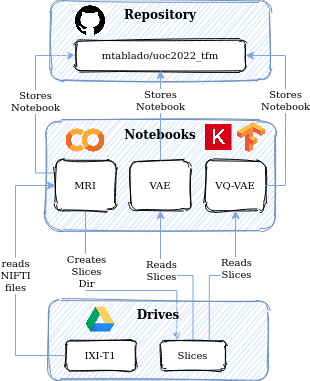
\includegraphics[]{images/tfm-environment.png}
    \caption[Environment and flows of information]{Environment and flows of information}
    \label{fig:environment}
\end{figure}

The project consists of 3 notebooks:

\begin{itemize}
    \item MRI which reads, processes and stores IXI images
    \item VAE which implements VAE model which uses pre-processed images
    \item VQ-VAE which implements VQ-VAE model which uses pre-processed images
\end{itemize}


\section{Phase 1: Analysis of MRI images dataset}

\subsubsection*{NIFTI protocol}

The NIFTI protocol stores the MRI scan images in 3D format with spatial information that allows the doctors to analyze images knowing the orientation along with some other metadata. Data is stored in vector-based fashion with voxel information.

This project is using the \cite{nibabel} library to load and process MRI images from nifti files. The library loads nifti files and retrieves an in-memory object with the image data containing slices in a 3-dimensional array. Accessing slices is then as easy as using the three indexes in the array, where you can easily get a slice by using the slice number from your chosen axis.

\subsubsection*{Loading images}
Extract 2D images: Load 3D images and extract 2D slices from the original dataset, which will be depicted with code.

After loading NIFTI images with the nibabel library \dots

\begin{figure}[ht]
    \centering
    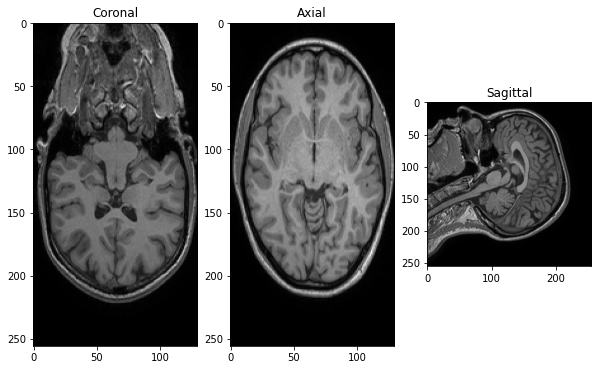
\includegraphics[width = 10cm, height = 6cm]{images/3-axis.png}
    \caption[]{Coronal, Axial and Sagittal images}
    \label{fig:3-axis}
\end{figure}

Images are loaded in the following shape:

\begin{itemize}
    \item 256 slices of Coronal or trasversal plane 
    \item 256 slices of Axial or horizontal plane
    \item 130 slices of Sagittal
\end{itemize}

\subsubsection*{Deciding what slices to use}

Looking at the three different slices in Figure \ref{fig:3-axis}, it is obvious that images have not been processed to show only the brain but the whole skull. The aim of the project is to create artificial brain images, not head ones. A model that would learn head images would require much more time and resources than for learning just the brain (which is not an easy task at all either).

While observing the BraTS \cite{brats} challenge dataset and project description, the skull stripping concept arise. Skull stripping consists on removing anything that does not pertain to brain or, in other words, extract the brain from the skull. 

\begin{figure}[ht]
    \centering
    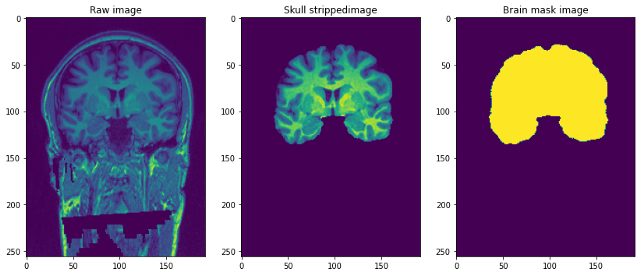
\includegraphics[width = 10cm, height = 6cm]{images/skull-stripped.png}
    \caption[]{Skull stripped image example; Source: Analytics Vidhya \cite{skullstripping} }
    \label{fig:skullstripped}
\end{figure}

This project cannot afford such implementation within the project scope. So, when deciding what slices to use, it became the only decision factor. It happened to be that the rest of considerations where just debatable and clearly much less important.

In conclusion, the noise that bones, eyes and the rest of the items visible in coronal and sagittal axis look very high compared to the axial slices in where, properly selected, slices will only show a surrounding skull bone.

Once that the axial slices were chosen, a sample of brain scans were visually analyzed to find a range of slices that could be used.

Figure \ref*{fig:slice160} shows a red line which bottom-up delimits  the range that goes from above the eyes to the top which is the range that excludes as much non-brain pixels as possible

\begin{figure}[ht]
    \centering
    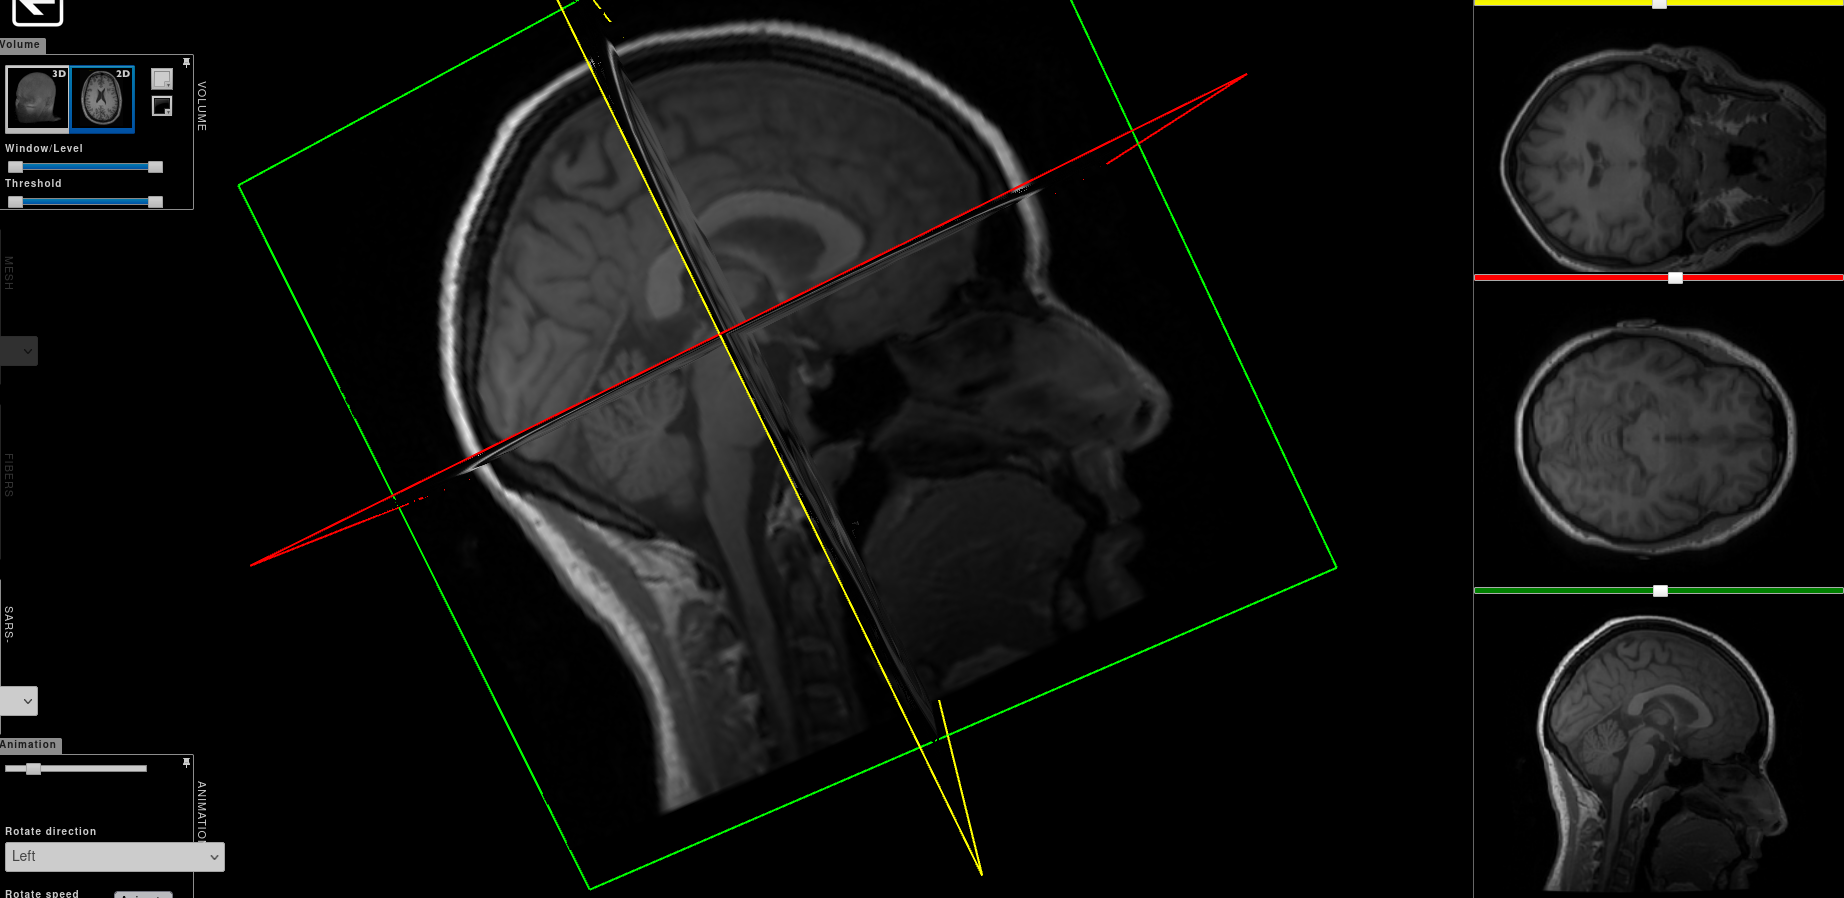
\includegraphics[width = 10cm, height = 6cm]{images/nifti-slice160.png}
    \caption[]{In red, slice 160 as bottom delimiter}
    \label{fig:slice160}
\end{figure}

Also, the slices closer to the top were also discarded to avoid higher heterogeneity on brain images (size and content). See Figure \ref*{fig:slice190}.

\begin{figure}[ht]
    \centering
    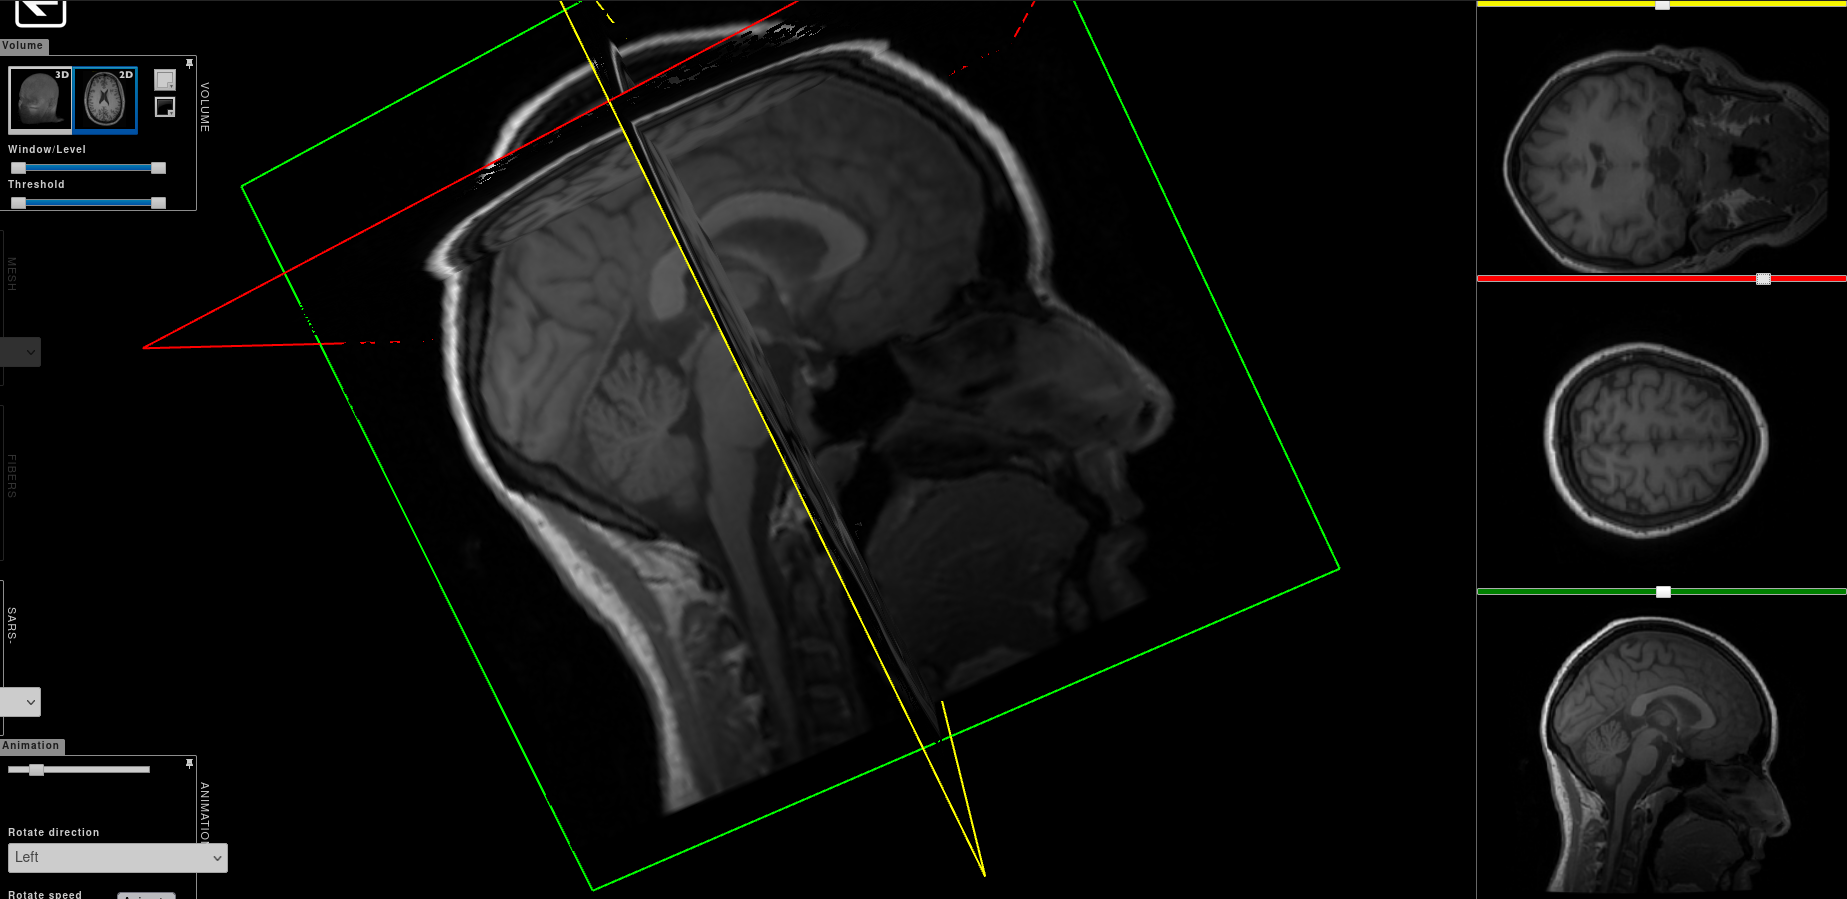
\includegraphics[width = 10cm, height = 6cm]{images/nifti-slice190.png}
    \caption[]{In red, slice 190 as top delimiter}
    \label{fig:slice190}
\end{figure}

It can be interpreted that 3D images are in use since 30 slices of each brain are used which constitue a 3D section of a brain. But, similarly, it could be interpreted that each and every slice of those 30 could happen to be data augmentation or different people with very similar brains.

\subsubsection*{Data Pre-processing and Data Augmentation}

Different pre-processing and data augmentation techniques were briefly evaluated to decide wheter if they would improve the model's results or not. Table \ref{table:preprocessing} shows the decisions made on each evaluated technique.

Overall, pre-processing actions that were feasible to implement in a timely manner were approved while those that could risk the project plan were discarded.

Also, data augmentation techniques that could result on unpredictable latent space results were initially discarded to be re-evaluated at a future work when the first results and conclusions would be available.

\begin{table}
    \centering
    \begin{tabular}{p{3cm}|p{2cm}|p{6cm}}
        \hline
        Technique & Decision & Justification \\
        \hline
        Gray scale & Approved & Applying gray scale to scans seems a natural choice and is usually applied on image processing \\
        Rescaling & Approved & Rescaling \acrshort{rgb} values from 0-256 to 0-1 that can be better handled by the model  \\
        Pixeling & Approved & Down-pixeling images from 256 to 128 which requires much less resources and without losing much quality \\
        Shear Intensity & Declined & Slanting images would distort the latent space leading to create distorted artificial images \\
        Shifts and Rotation & Declined & Similar to shear intensity shifting images is seen as a method not accurate for MRI processing as MRI images will not appear shifted in any prediction phase \\
        Add Noise & Declined & Adding noise is interesting for improving results and key to allow model transfering to other datasets obtained with different scanners and their settings or image quality. It was declined due to time constraints. \\
        \hline
    \end{tabular}
    \caption{Pre-processing techniques decissions table}
    \label{table:preprocessing}
\end{table}

% To place the table.
\newpage

\subsubsection*{Storing data}

In order to separate image loading from model training into different steps, selected 2D images are stored in \acrshort{png} format after being pre-processed. 

The images are stored in 2 different directories spliting the dataset into 90\% for training and 10\% for test subsets resulting in 16.268 and 1.162 images respectively.
\section{Phase 2: MR Images creation}

\subsection{Variational Autoencoder}

The source code of the implemented VAE can be found at \href{https://github.com/mtablado/uoc2022_tfm/blob/main/vae.ipynb}{vae.ipynb} file inside the project repository and it is inspired by Variational Autoencoder \cite{vaekeras} keras example.

\begin{figure}[ht]
    \centering
    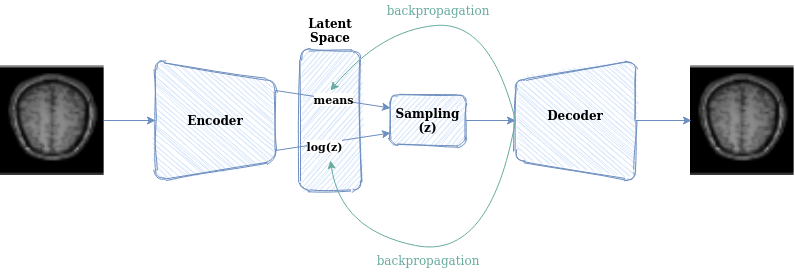
\includegraphics[width = 16cm, height = 6cm]{images/vae.png}
    \caption[]{Diagram of Implemented VAE Architecture}
    \label{fig:vaearch}
\end{figure}

The encoder consists of a \acrfull*{cnn} that uses the preprocessed brain slices images as input and then two vectors that form the latent space, which has been sized to store 1024 attributes. \acrshort*{cnn} implementation is described later in a dedicated section.

Encoder output vectors are:

\begin{itemize}
    \item A 1024-dimensional vector of means ($\mu$), and
    \item a 1024-dimensional vector of standard deviations (z) as $log(z)$ to make sure they are positive.
\end{itemize}
 
Then those vectors are sampled and feeded into the decoder to reconstruct the \acrshort{mri}. Backpropagation is applied to correct latent space issues and let the model be more accurate.

To implement above architecture in Keras, a new model was created by overriding the Keras Model abstract class and implementing the methods that the interface requires. So, specific methods are coded to process each and every train step and the metrics property is overriden to store the training loss, the reconstruction loss and the Kullback-Leibler divergence data.

The training method calculates the reconstruction loss and the KL divergence. Then, their values are aggregated to result in the training loss value.

\begin{equation}
    Training Loss = Reconstruction Loss + KL Divergence
\end{equation}

The reconstruction loss measures how close the encoder input and the encoder output are by calculating the \acrshort{mse} of the difference between images. On the other hand the KL-Divergence measures the distance between two probability distributions. So, minimizing the KL loss in this case means ensuring that the learnt means and variances are as close as possible to those of the target (normal) distribution.

The latent space of the VAE is usually a Gaussian distribution. Gaussian distribution is also used here since it has very good computational properties. 

The sampling process is implemented as an encoder Keras Layer which takes both vectors and samples with a formula that aggregates the mean and the variance which adjusted with a random factor.


\subsubsection*{The KL-Divergence issue}

As introduced in \ref*{sec:imploverview} overview section, some deviations from the project happened. The KL-Divergence interpretation and calculation was (and remains) a problem. Contrary to what should happen, instead of decreasing, the KL-Divergence metric increases along the epochs. 

Several calculation formulas for KL-Divergence were tested with little result changes (they are commented in at source file). 

The best model accuracy comes at maximizing the ELBO, which happens when you minimize both reconstruction loss and KL\-Divergence.

Despite the KL-Divergence issue, the ELBO improves in each step thanks to the higher minimization of the reconstruction loss

\begin{equation}
    \left\lvert Reconstruction Loss_i - Reconstruction Loss_{i-1} \right\rvert > \left\lvert KL Divergence_i - KL Divergence_{i-1} \right\rvert
\end{equation}
 
This casualty is allowing the model to keep learning.

This issue inclined the project to create a secondary approach, train also a \acrshort*{vqvae} model to compare results which is describe in the following section, since the time constraint did not allow the project to keep investigating on this issue.

\subsection{Vector-Quantized Variational Autoencoder}

The source code of this section can be found at \href{https://github.com/mtablado/uoc2022_tfm/blob/main/vq-vae.ipynb}{vq-vae.ipynb} file inside the project repository and it is inspired by Vector-Quantized Variational Autoencoder \cite{vqvaekeras} keras example, which code was used as starting point.

\begin{figure}[ht]
    \centering
    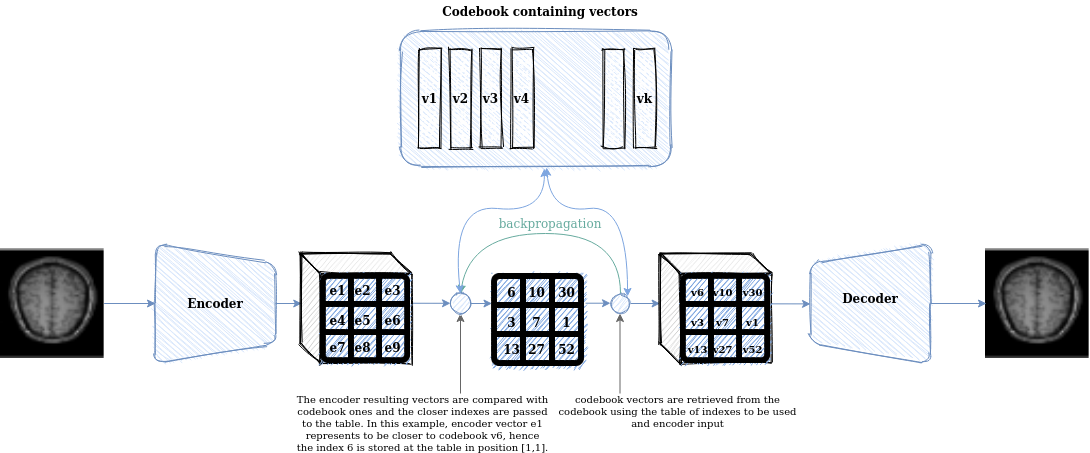
\includegraphics[width = 16cm, height = 8cm]{images/vq-vae.png}
    \caption[]{Diagram of Implemented VQ-VAE Architecture}
    \label{fig:vqvaearch}
\end{figure}

As VAE, \acrshort*{vqvae} use \acrshort*{cnn} but, in this case, the encoder generates a set of vectors with discrete representations (instead of continuous like VAE)  that is 
During training phase VQ-VAE creates a codebook of vectors which are also learnable and predictable. Once that a new image is processed, the encoder output vector of z is compared with the codebook vectors and the one closer to it is used later as the input of the decoder. Proximity between vectors is calculated with the L2-norm.

The resulting indexes are stored into a set that then serves as the indexing object to build a new set of vectors that will be used as decoder input.

To do above-mentioned steps, a Vector Quantizer object (a new type of Keras Layer) was created to select the quantized vectors from the latent space which are closer to the encoder output vectors and then, those quantized vectors will be used as decoder inputs.

To implement above architecture in Keras, as like for VAEs and along with the Vector Quantized object, a new model was created by overriding the Keras Model abstract class and implementing the methods that the interface requires. So, specific methods are coded to process each and every train step and the metrics property is overriden to store the total loss, the reconstruction loss and the VQ loss.

The training method calculates the reconstruction loss and the VQ loss and uses them to calculate the training loss (total training here) with the following formula:

\begin{equation}
    Total Loss = Reconstruction Loss + \sum (VQ losses)
\end{equation}

\subsection{CNN Network Architectures}

The implemented \acrshort{cnn} is based on Context-encoding Variational Autoencoder for Unsupervised Anomaly Detection paper \cite{cevaemodel} in where Zimmerer et al. describe it as: 

\begin{quote}
    For the encoder and decoder networks, we chose fully convolutional networks with five 2D-Conv-Layers and 2D-Transposed-Conv-Layers respectively with CoordConv, kernel size 4 and stride 2, each layer followed by a Leaky-ReLU non-linearity. The encoder and decoder are symmetric with 16, 64, 256, 1024 feature maps and a latent variable size of 1024
\end{quote}

Figure \ref{fig:cnnencoderoutput} shows the encoder model summary output after compiling the model. It is truncated to show only CNN-related layers removing VAE or VQ-VAE specific layers. Full output can be checked at Figures \ref{fig:cnnvaeencoderoutput} and \ref{fig:cnnvqvaeencoderoutput}

\begin{figure}[ht]
    \centering
    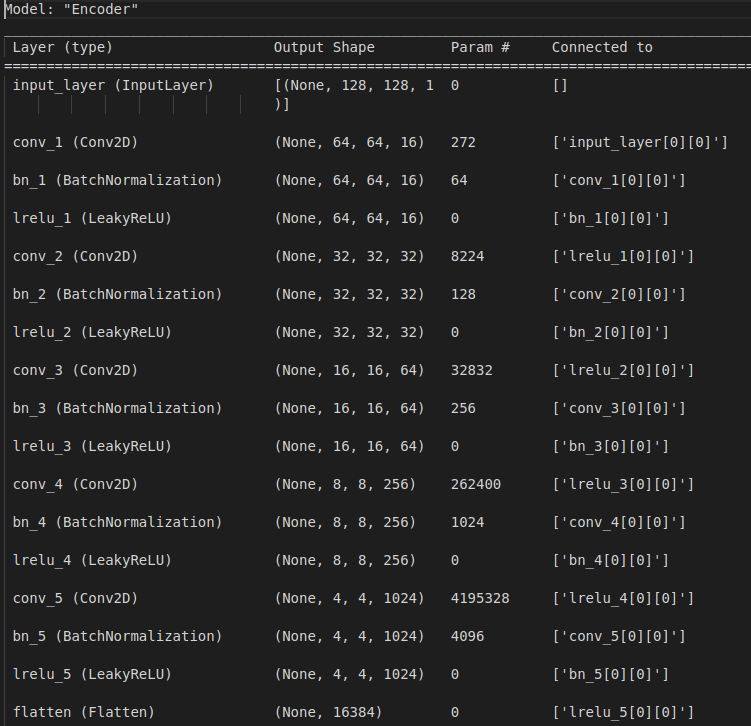
\includegraphics[width = 14cm, height = 8cm]{images/cnn-encoder-output.png}
    \caption[]{CNN Encoder model summary output}
    \label{fig:cnnencoderoutput}
\end{figure}

The input size of the \acrshort*{cnn} is [128,128,1] which are the 128 pixels resulting of the preprocessing downsampling and the usage of 1 channel for the gray scale data.

Figure \ref{fig:cnndecoderoutput} shows the decoder model summary output after compiling the model.

\begin{figure}[ht]
    \centering
    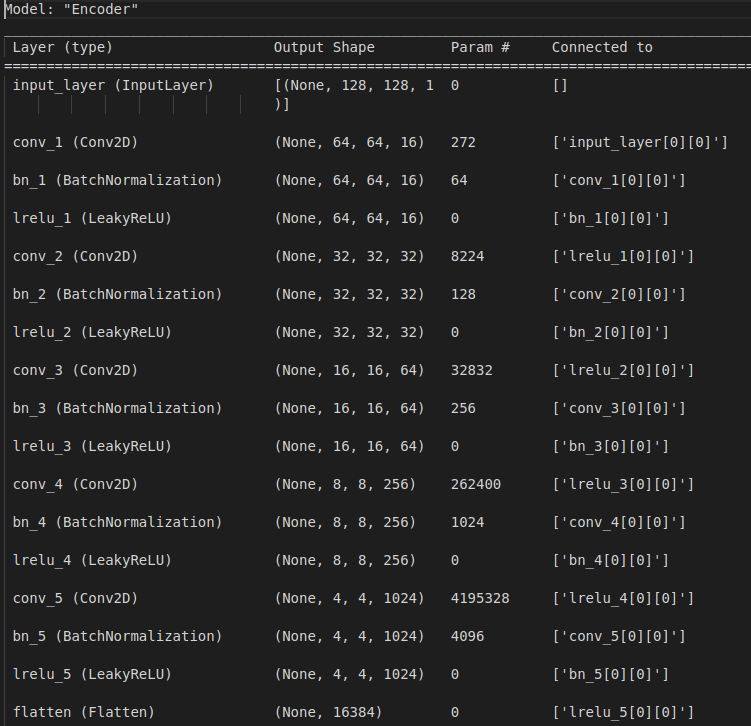
\includegraphics[width = 14cm, height = 8cm]{images/cnn-encoder-output.png}
    \caption[]{CNN Decoder model summary output}
    \label{fig:cnndecoderoutput}
\end{figure}

Both of the above-described VAE and VQ-VAE models use this network architecture to encode and decode images where different steps/layers are put in between them to implement the differences of the two models.

\newpage

\begin{figure}[ht]
    \centering
    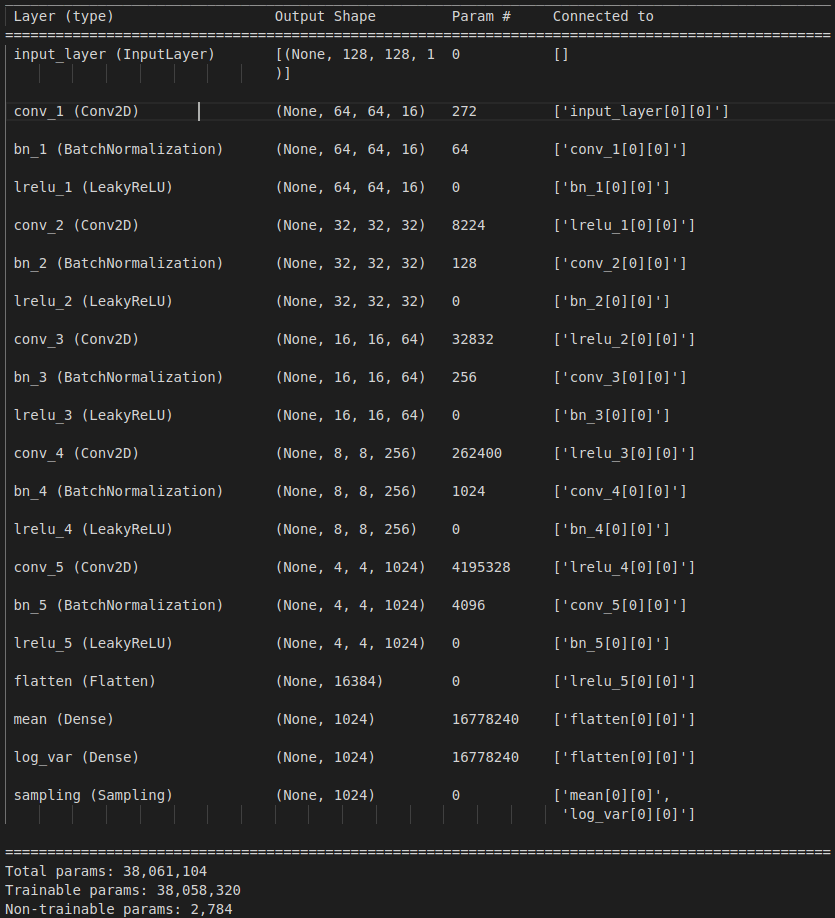
\includegraphics[width = 14cm, height = 12cm]{images/cnn-vae-encoder-output.png}
    \caption[]{CNN VAE encoder model summary output}
    \label{fig:cnnvaeencoderoutput}
\end{figure}

\newpage

\begin{figure}[ht]
    \centering
    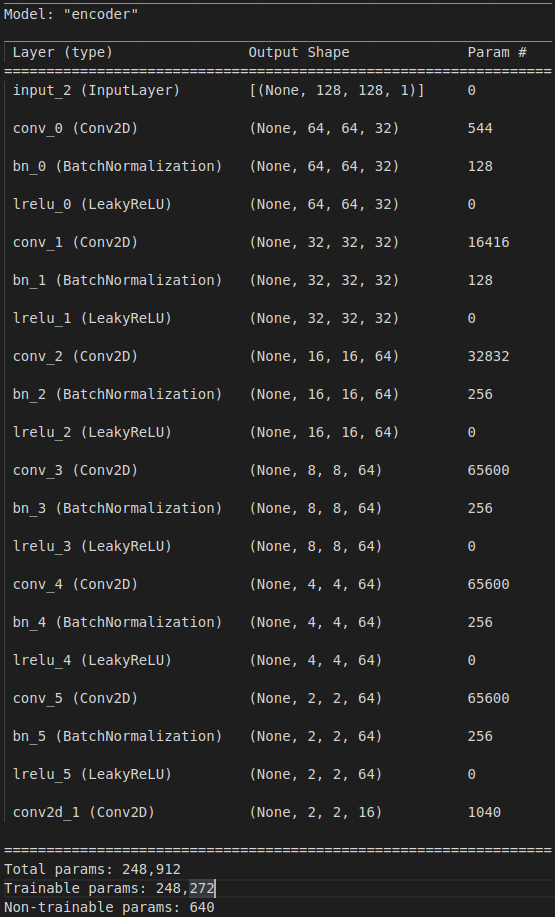
\includegraphics[width = 14cm, height = 12cm]{images/cnn-vqvae-encoder-output.png}
    \caption[]{CNN VQ-VAE encoder model summary output}
    \label{fig:cnnvqvaeencoderoutput}
\end{figure}

\subsubsection{Hidden Layers}

As described in this section, the implemented \acrshort{cnn} is based on Context-encoding Variational Autoencoder for Unsupervised Anomaly Detection paper \cite{cevaemodel} in where Zimmerer et al. describe it as: 

\begin{quote}
    For the encoder and decoder networks, we chose fully convolutional networks with five 2D-Conv-Layers and 2D-Transposed-Conv-Layers respectively with CoordConv, kernel size 4 and stride 2, each layer followed by a Leaky-ReLU non-linearity. The encoder and decoder are symmetric with 16, 64, 256, 1024 feature maps and a latent variable size of 1024
\end{quote}

In project's \acrfull{cnn}, a Normalization neuron is added between them resulting in the following composite:

\begin{itemize}
    \item Convolutional neuron (Conv2D or Conv2DTranspose) 
    \item Normalization neuron (BatchNormalization)
    \item ReLu neuron (LeakyReLu)
\end{itemize}

The convolutional layer is paremetrized with 4 kernels, stride 2 and padding 0. The kernel size aims to avoid the network learning too fast, while using stride 2 to lower the training resources needed and train faster.

According to Martin Riva \cite{batchnorm} "Batch Norm is a normalization technique done between the layers of a Neural Network instead of in the raw data. It is done along mini-batches instead of the full data set. It serves to speed up training and use higher learning rates, making learning easier. the standard deviation of the neurons' output.". The project is loading raw data in batches which are normalized as a preparation step, however, normalizing data between each layer might help.

ReLu neuron is usually applied in Deep Learning (and so it is in the project) right after every convolutional neuron to remove linearity since, basically, all the previous operations are linear. 

\subsection{Flow from directory}

An interesting implemented feature is the ability to use an interator for image loading which is in fact called by the VAE and VQ-VAE models. So that in each iteration a batch of images is loaded in memory and ready to be used within the model.

Aligning the model batch size with the iterator batch size avoids unnecessary calls and more importantly tunes memory usage while training the models.

The flow from directory method is also the responsible to downsample pixeling since images are stored with 256 and the model expects only 128.

\subsection{Creating artificial images from latent space}

To create artificial images from the latent space the decoder input must be generated. As explained, the decoder expects an object from the latent space, which means that 1024 values are expected in the normal Gaussian distribution. This is randomly generated with NumPy library and its \href{https://numpy.org/doc/stable/reference/random/generated/numpy.random.normal.html}{numpy.random.normal} function.
\newpage 

\subsection{Results and Experiments}

\subsubsection{Final Results}

The described implemented architecture of VAE and VQ-VAE models results show that the models are learning but they are not able to create images that could be interpreted as real.

\begin{figure}[ht]
    \centering
    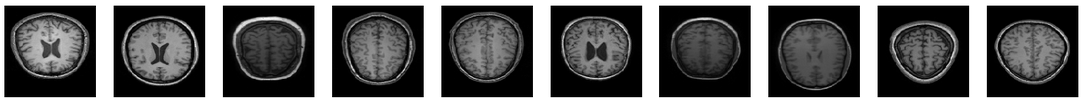
\includegraphics[width = 17cm]{images/mri-real-images.png}
    \caption[Real MR Images]{Real MR Images}
    \label{fig:mri-real-images}
\end{figure}

\begin{figure}[ht]
    \centering
    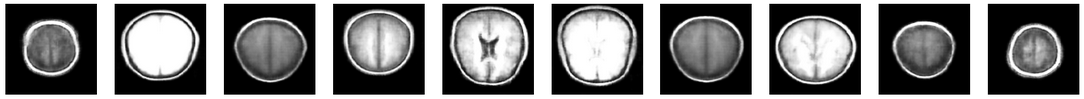
\includegraphics[width = 17cm]{images/vae-brains-results.png}
    \caption[VAE Reconstructed Images]{VAE Reconstructed Images}
    \label{fig:vae-brains-results}
\end{figure}

\begin{figure}[ht]
    \centering
    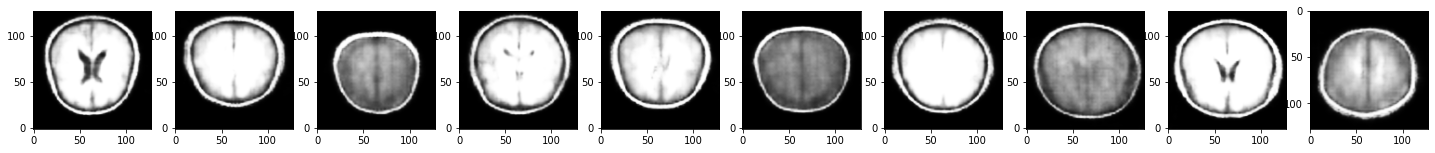
\includegraphics[width = 17cm]{images/vqvae-brains-results.png}
    \caption[VQ-VAE Reconstructed Images]{VQ-VAE Reconstructed Images}
    \label{fig:vqvae-brains-results}
\end{figure}

Reconstructed images are slices that were created using the test data. They were created using the output of the encoder as the decoder input not artificially generated.

Note that real images shown in Figure \ref{fig:mri-real-images} do correlate with images shown in Figures \ref{fig:vae-brains-results} and \ref{fig:vqvae-brains-results}.

\begin{figure}[ht]
    \centering
    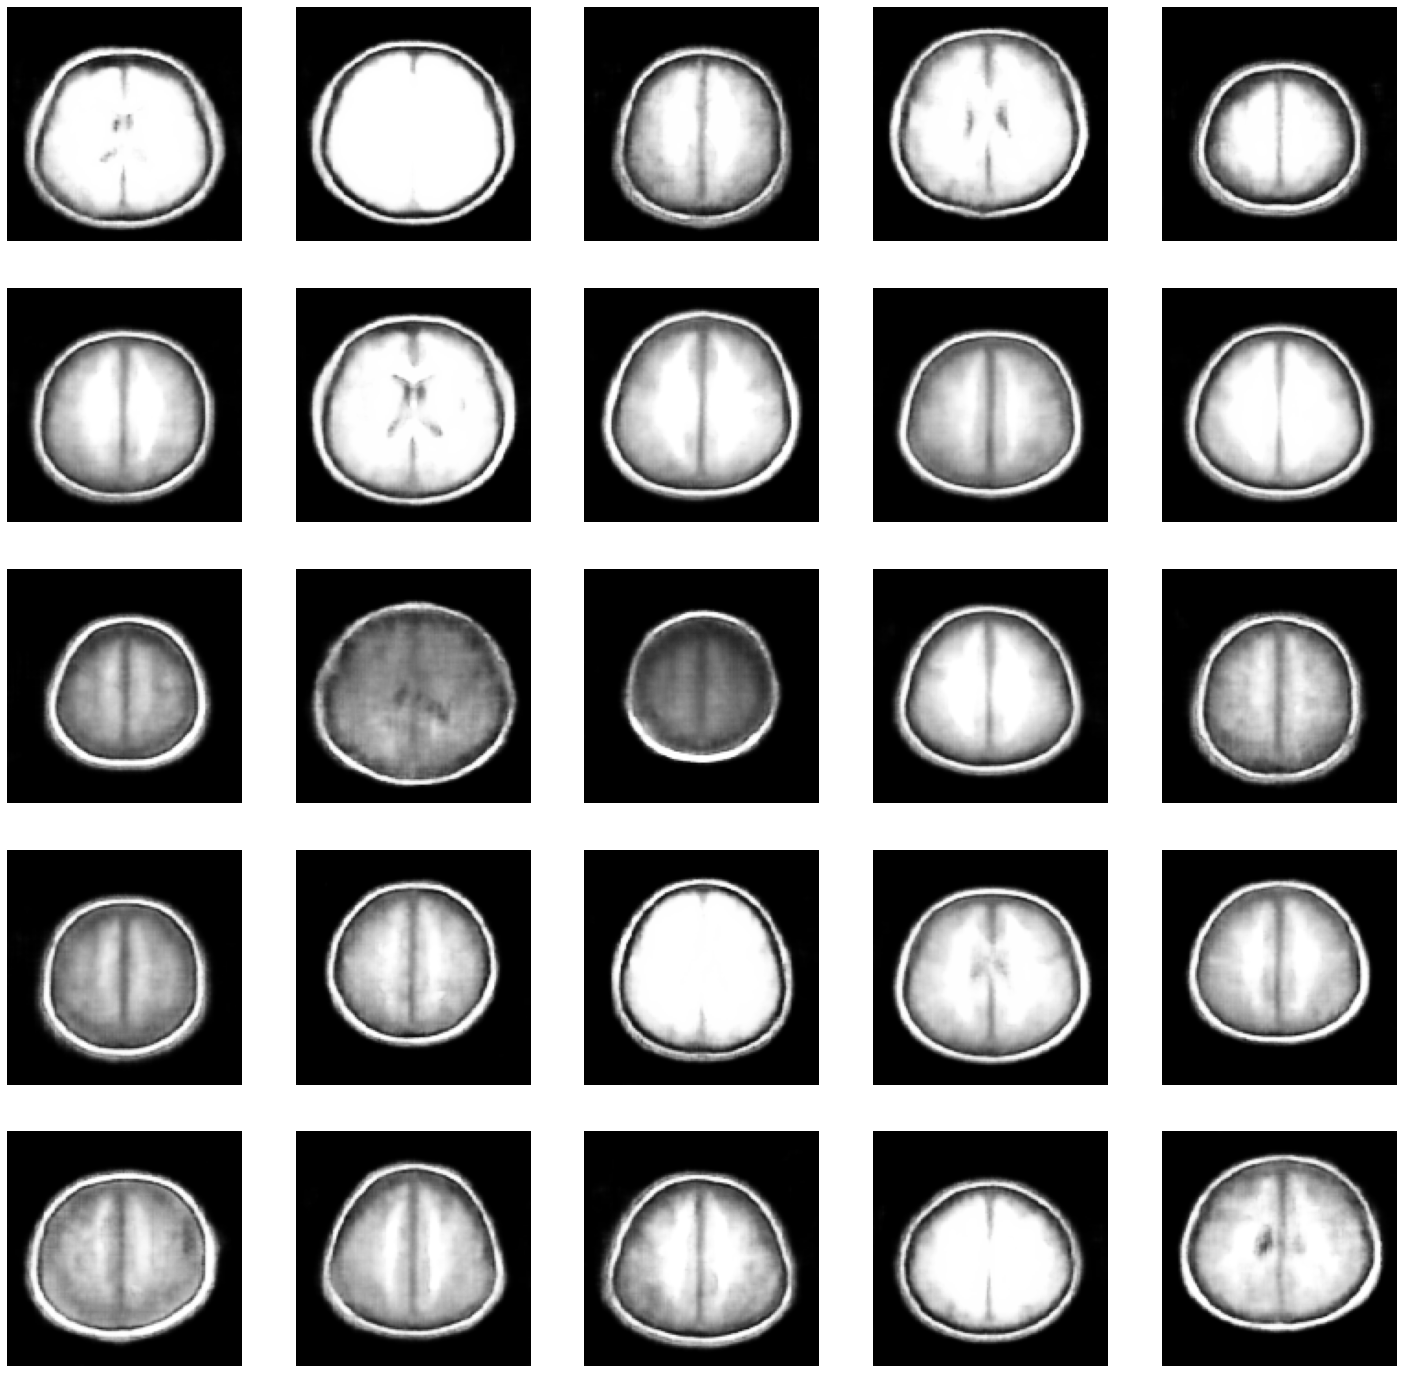
\includegraphics[width = 17cm]{images/vae-brains-results-from-latent-space.png}
    \caption[Artificial VAE images created from latent space]{Artificial VAE images created from latent space}
    \label{fig:vae-images-from-latent-space}
\end{figure}

Looking at technical results, the models seem to learn very slowly but they keep learning even at 500 epochs so the models' limits are yet to be discovered. On the other hand, as explained in dedicated section, VAE model shows an issue with the KL Divergence, it becomes higher over epochs while it must be decreased.

\begin{figure}[ht]
    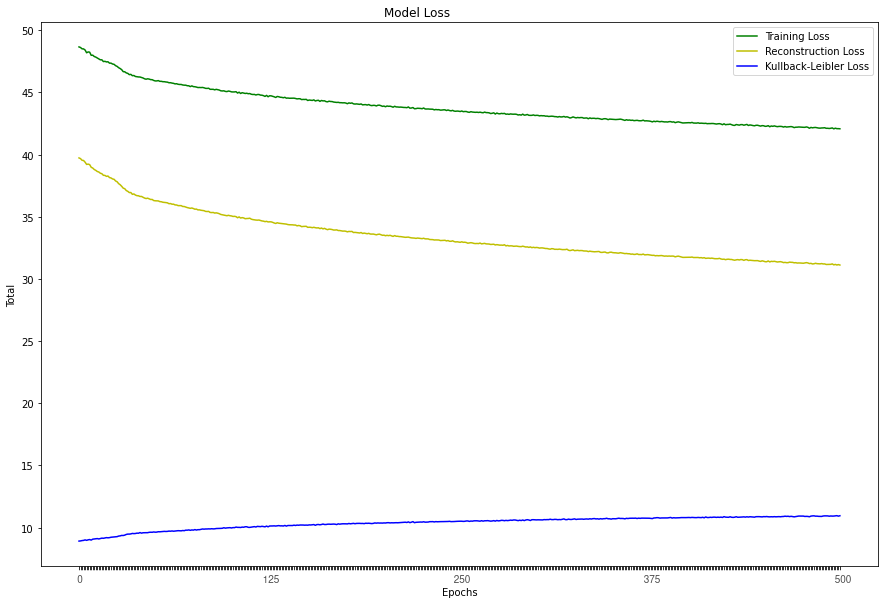
\includegraphics[width = 17cm]{images/vae-loss-results.png}
    \caption[VAE Training loss]{VAE Training loss}
    \label{fig:vae-training-loss}
\end{figure}

\begin{figure}[ht]
    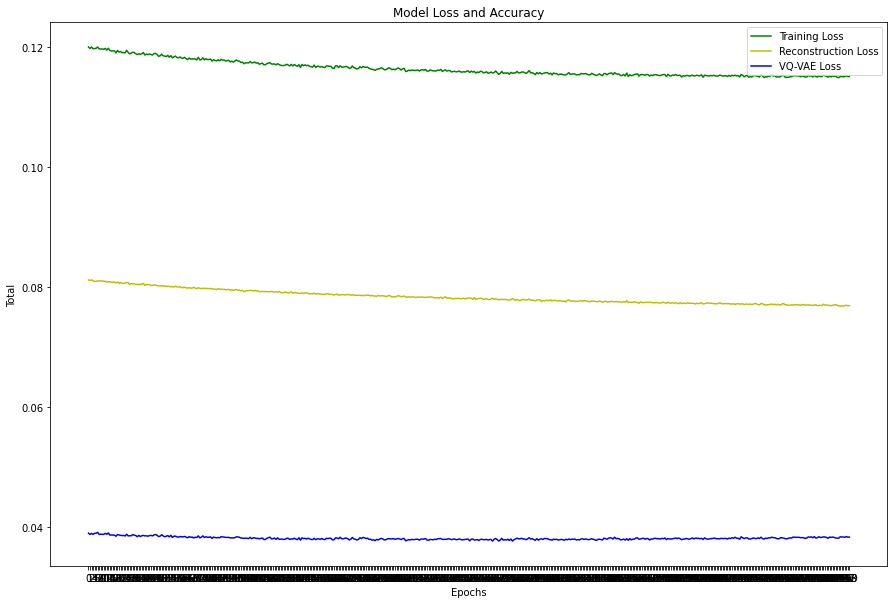
\includegraphics[width = 17cm]{images/vqvae-loss-results.png}
    \caption[VQ-VAE Training loss]{VQ-VAE Training loss}
    \label{fig:vqvae-training-loss}
\end{figure}


% Make sure floats (figures) are placed before new section
\FloatBarrier

\subsubsection{Experiments}

The project methodology determined that after every task a fast status analysis was assessed. The reason to do so was the research nature of the project that required continuous evalution on the process and results.

Most of the experiments were executed during the creation of images phase. Whereas the resulting pre-process tasks were overall clear due to  \acrshort{mri} slices deep study, executed at the analysis phase of the project, the creation of images required analysis and implementation cycles since at the analysis phase of the project VAEs' theory was checked but the implementation tasks were not.

Instead of creating it from scratch, a simple \acrfull{cnn} that is used to show VAE example on MNIST \cite{mnist} digits was picked. It was used to test the code functionality only, results were not important and they were discarded. 

Once that the functionality was proved to work, the 5-block network was implemented with the following features (it details only the features that vary from the final model):

\begin{itemize}
    \item 128, 64, 32, 16 and 8 dimensions and a latent space of 200
    \item kernel size was 3
    \item trained on 30 epochs only
    \item 256 pixels
\end{itemize}

Producing the images shown in Figure \ref*{fig:vae-k3-brains-30-epochs} and losses shown in Figure \ref*{fig:vae-k3-loss-30-epochs}

\begin{figure}[ht]
    \centering
    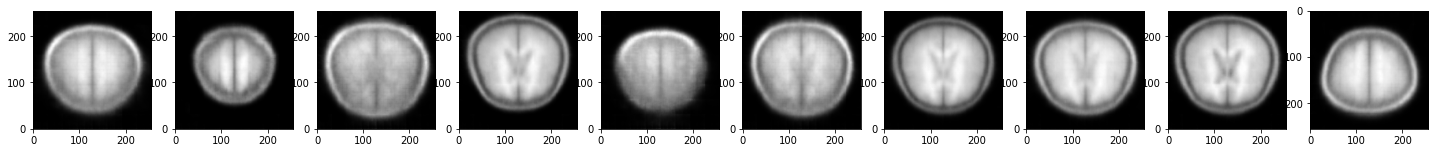
\includegraphics[width = 17cm]{images/vae-k3-brains-30-epochs.png}
    \caption[VAE Results on experiments I]{VAE Results on experiments I}
    \label{fig:vae-k3-brains-30-epochs}
\end{figure}

\begin{figure}[ht]
    \centering
    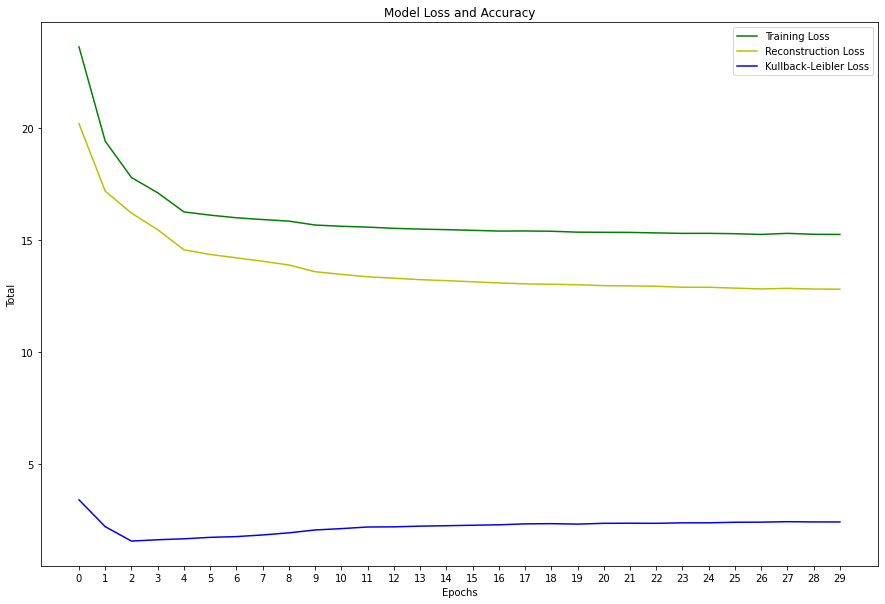
\includegraphics[width = 14cm, height=8cm]{images/vae-k3-loss-30-epochs.png}
    \caption[VAE Losses on experiments I]{VAE Losses on experiments I}
    \label{fig:vae-k3-loss-30-epochs}
\end{figure}

At that time, since results on images were not ideal the new approach was created in order to double-check if the kl-divergence issue could be the reason for not getting better results. A VQ-VAE implementation was created along with an extra sixth layer added at the begining of the encoder, looking for a slower learning approach. The VQ-VAE implementation with 6 layers produced the images shown in Figure \ref*{fig:vqvae-6layers-30-epochs} and losses shown in Figure \ref*{fig:vqvae-6layers-loss-30-epochs}

\begin{figure}[ht]
    \centering
    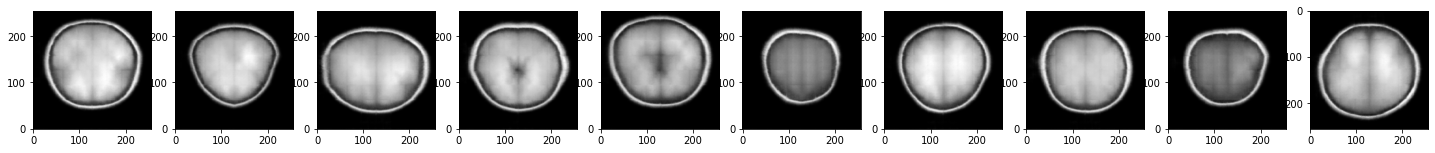
\includegraphics[width = 17cm]{images/vqvae-6layers-30-epochs.png}
    \caption[VQ-VAE Results on experiments II]{VQ-VAE Results on experiments II}
    \label{fig:vqvae-6layers-30-epochs}
\end{figure}

\begin{figure}[ht]
    \centering
    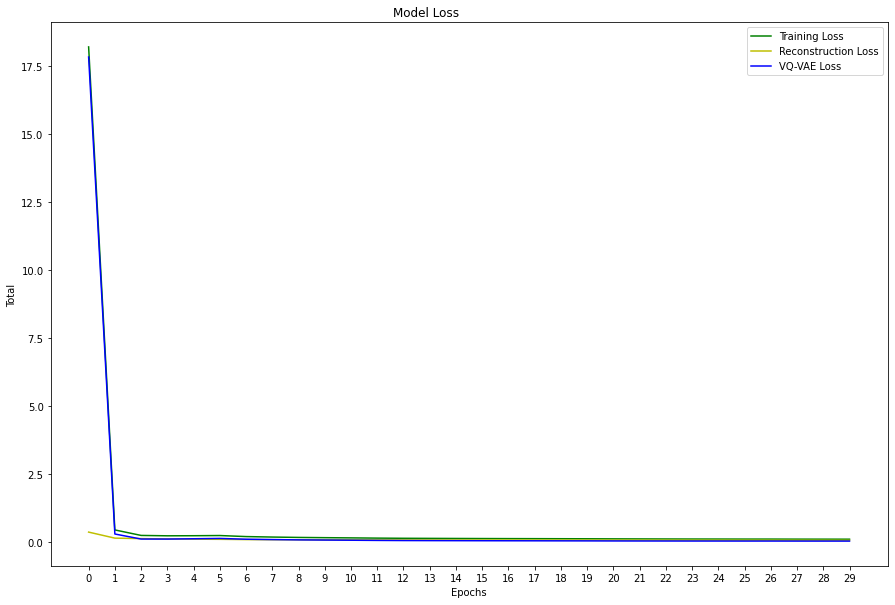
\includegraphics[width = 14cm, height=8cm]{images/vqvae-6layers-loss-30-epochs.png}
    \caption[VQ-VAE Losses on experiments II]{VQ-VAE Losses on experiments II}
    \label{fig:vqvae-6layers-loss-30-epochs}
\end{figure}

Then, after checking that VAE and VQ-VAE produced similar results it was decided to look into different angles of potential improvements and the downsampling of pixels experiment was chosen to be next. Along with downsampling, the number of epochs was increased to 200.

VAE Produced the images shown in Figure \ref*{fig:vae-brains-128pixels-200epochs} and losses shown in Figure \ref*{fig:vae-loss-128pixels-200epochs}

\begin{figure}[ht]
    \centering
    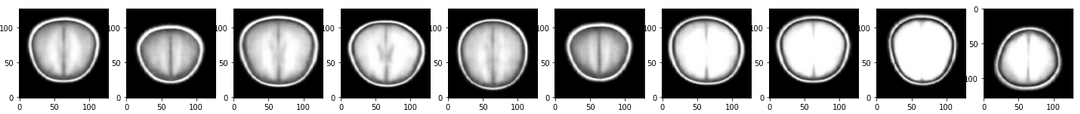
\includegraphics[width = 17cm]{images/vae-brains-128pixels-200epochs.png}
    \caption[VAE Results on experiments III]{VAE Results on experiments III}
    \label{fig:vae-brains-128pixels-200epochs}
\end{figure}

\begin{figure}[ht]
    \centering
    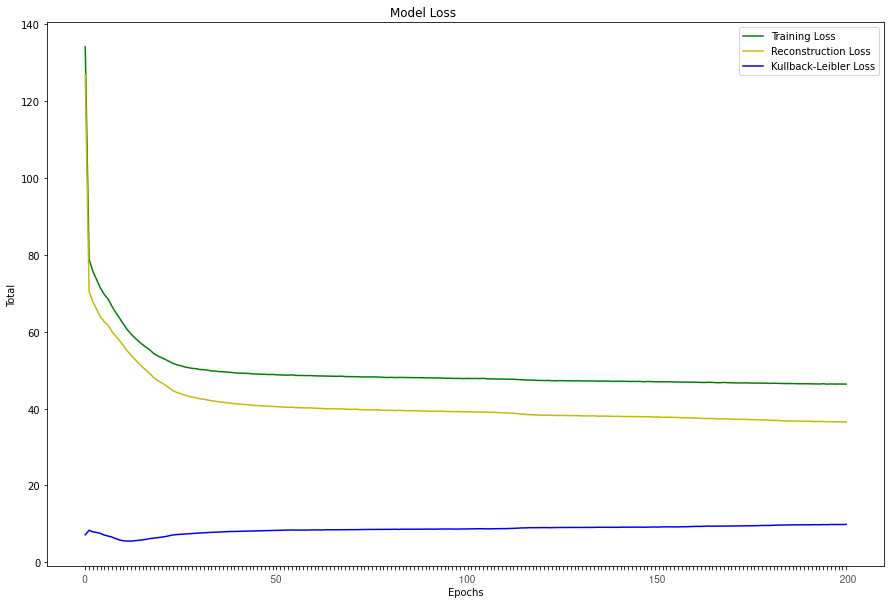
\includegraphics[width = 14cm, height=8cm]{images/vae-loss-128pixels-200epochs}
    \caption[VAE Losses on experiments III]{VAE Losses on experiments III}
    \label{fig:vae-loss-128pixels-200epochs}
\end{figure}

After that, some other parameters changes were tested with no remmarkable results compared to the latest results obtained. Tested parameters were learning rates 0.0001, 0.0005 and kernel size 3, trained on 500 epochs.
